\section{Manual}
This section will give a detailed description of how the program should and can be used. The first part discusses the setup and how to use the GUI. In the second part output data handling is discussed.
	\subsection{GUI}
The GUI consists of a window with four tabs. The first tab provides a list of elements, or chemicals, that can be used for simulation as seen in fig \ref{fig:mat_tab}. Note that not all of these elements are suitable for the Lennard-Jones potential. After each element, their respective crystal structures are written. To choose an element simply click on it and then select the next tab.
\begin{figure}[h!]
	\centering
	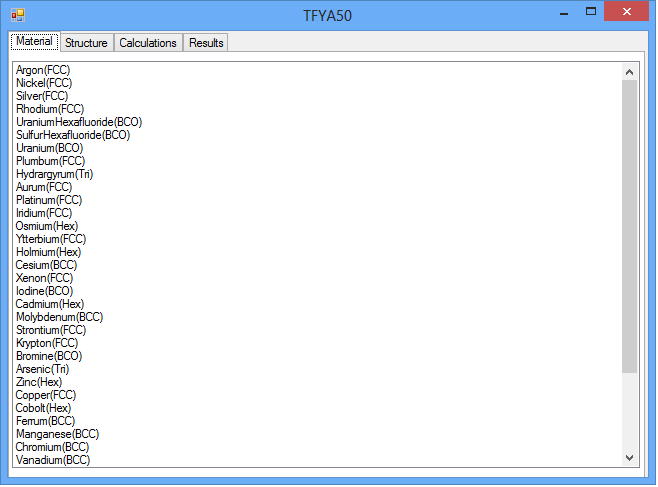
\includegraphics[width=0.7 \textwidth]{mat_tab.png}
	\caption{Interface for choosing material}
	\label{fig:mat_tab}
\end{figure}
In the second tab, the Lennard-Jones parameters, the crystal structure and the spatial dimensions can be specified. See figure \ref{fig:struct_tab}. The default values shown depend on the element that was chosen in the previous step. The pre-set values can be changed according to the user's wishes.
\begin{figure}[h!]
	\centering
	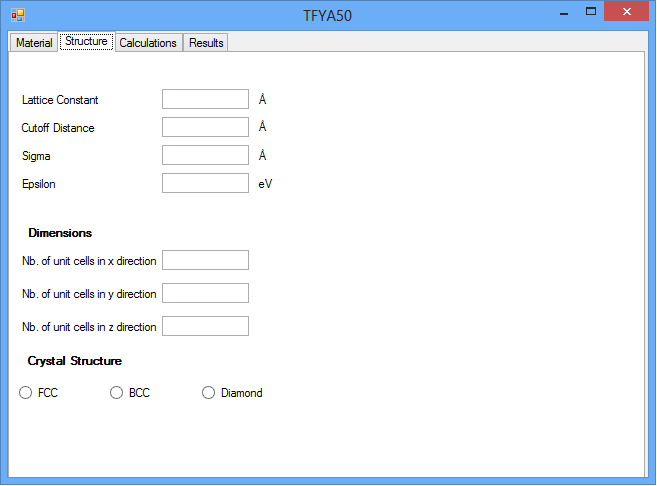
\includegraphics[width=0.7\textwidth]{struct_tab.png}
	\caption{Interface for setting material properties}
	\label{fig:struct_tab}
\end{figure}

The third tab consists of the simulation options. An overview is given in figure \ref{fig:calc_tab}. 
\begin{description}
	\item[Start calculations after \#timesteps] is the value at which point the average properties will start to accumulate
	\item[Run for \#timesteps] is the total number of timesteps that the simulation will be carried out over. 
	\item[Timestep size] is how long each time step is in femtoseconds. This value multiplied by the total number of timesteps is the total runtime in femtoseconds. 
	\item[Include visualization] will when checked, make the program produce a Matlab file where the atomic movements can be visualized.
	\item[Save visualization every \#timestep] determines how often visualization data will be saved to the HDD.
	\item[Save data every \#timestep] determines how often the properties data will be saved to the HDD.
	\item[Thermostat] will when checked activate the thermostat and an option to set the collision rate will also be given.
	\item[Collision rate] is set to a number between 0 and 1 and is the probability for an atom to collide with the thermostat heat bath.
	\item[Temperature] is the starting temperature of the simulation. the atoms initial velocity will be scaled according to this. It will also be the temperature of the thermostat heat bath. The unit is K.
	\item[Use periodic boundary conditions] will when checked simulate the sample as continuous in the chosen directions. If boundary conditions are set an atom drifting away will jump over to the other side. By unchecking these surface simulations may be conducted.
\end{description}
\begin{figure}[h!]
	\centering
	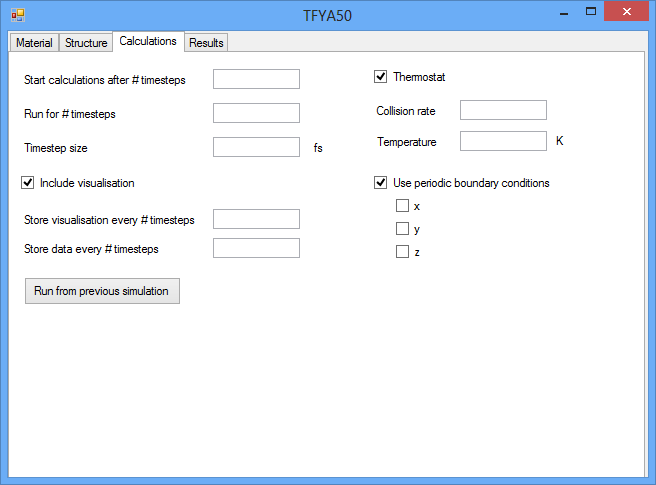
\includegraphics[width=0.7\textwidth]{calc_tab.png}
	\caption{Interface for setting calculation properties}
	\label{fig:calc_tab}
\end{figure}
	
The fourth and last tab is for starting the simulation and it will also provide the user with data on the simulation, as well as presenting the average values for the listed properties after simulation is completed. See figure \ref{fig:res_tab}.
\begin{figure}[h!]
	\centering
	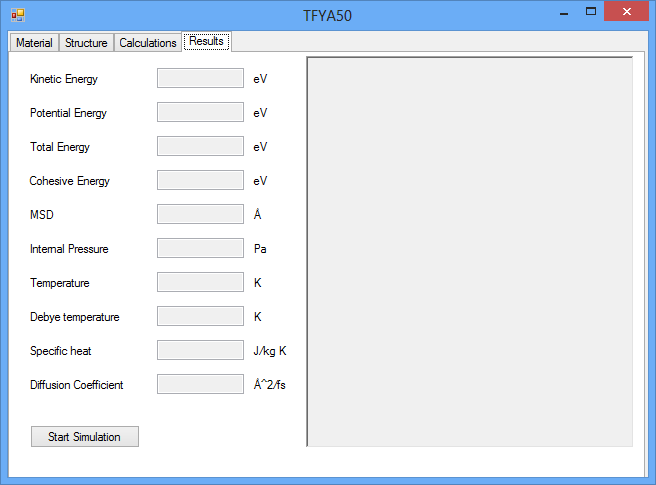
\includegraphics[width=0.7\textwidth]{res_tab.png}
	\caption{Interface for starting simulation and showing results}
	\label{fig:res_tab}
\end{figure}

The GUI is locked for the duration of the simulation. When it's done a notification appears and the GUI is unlocked. After running a simulation to the end, a back2back file is produced to allow for multiple runs from the last state. In tab 3 (figure \ref{fig:calc_tab}) simply choose ''Run from previous simulation'' and choose the desired saved file.

Since the program saves data to files with the same name for all runs, the user needs to change name for the ''back2back.txt'', ''toto.txt'' and ''titi.txt'' files or move them to a separate folder.

\subsection{Matlab}
All data files are saved in as simple tab delimited text files, so visualization of the movement and the properties may be conducted in a program of the user's choice, however Matlab is the recommended choice. There are two Matlab files provided with the program that will take the data from ''toto.txt'' and ''titi.txt'' to calculate and plot the average values, and do the visualization. To do so, launch Matlab and locate the folder with the Matlab files along with the .txt-files. In Matlab, to plot the data, run the command ''plot\_data('toto.txt','\textbackslash{}t')'', where ''toto.txt'' is the name of the datafile and \textbackslash{}t is the delimiter. ''toto.txt'' is the default name for the properties data, but the user may enter another name if the name of the data files have been changed. After running the command, nine plots are produced. For the visualization part, simply run ''plot\_atoms()'' and the visualization will be loaded from the ''titi.txt'' file in the project folder.
